Berechnen Sie den Flächeninhalt des Polygons mit den Ecken
\begin{center}
\begin{tabular}{ll}
\begin{minipage}{0.45\hsize}
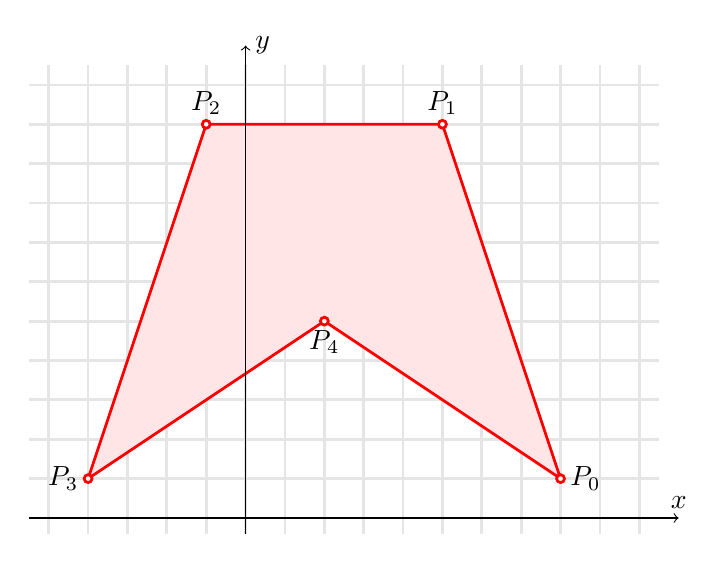
\begin{tikzpicture}[scale=0.5]
\coordinate (P0) at (8,1);
\coordinate (P1) at (5,10);
\coordinate (P2) at (-1,10);
\coordinate (P3) at (-4,1);
\coordinate (P4) at (2,5);
\foreach \x in {-5,-4,...,10}{
\draw[color=gray!20,line width=1pt] ({\x},-0.4)--({\x},11.5);
}
\foreach \y in {1,2,...,11}{
\draw[color=gray!20,line width=1pt] (-5.5,{\y})--(10.5,{\y});
}
\fill[color=red!10] (P0)--(P1)--(P2)--(P3)--(P4)--(P0);
\draw[color=red,line width=1pt] (P0)--(P1)--(P2)--(P3)--(P4)--(P0);
\draw[line width=1pt,color=red,fill=white] (P0) circle[radius=0.1] {};
\draw[line width=1pt,color=red,fill=white] (P1) circle[radius=0.1] {};
\draw[line width=1pt,color=red,fill=white] (P2) circle[radius=0.1] {};
\draw[line width=1pt,color=red,fill=white] (P3) circle[radius=0.1] {};
\draw[line width=1pt,color=red,fill=white] (P4) circle[radius=0.1] {};
\draw[->] (-5.5,0)--(11,0) coordinate[label={above:$x$}];
\draw[->] (0,-0.4)--(0,12) coordinate[label={right:$y$}];
\node at (P0) [right] {$P_0$};
\node at (P1) [above] {$P_1$};
\node at (P2) [above] {$P_2$};
\node at (P3) [left] {$P_3$};
\node at (P4) [below] {$P_4$};
\end{tikzpicture}
\end{minipage}&%
\begin{minipage}{0.3\hsize}
\[
\begin{aligned}
P_0&=(8,1)\\
P_1&=(5,10)\\
P_2&=(-1,10)\\
P_3&=(-4,1)\\
P_4&=(2,5)\\
P_8&=P_0
\end{aligned}
\]
\end{minipage}
\end{tabular}
\end{center}

\thema{Flächeninhalt}

\begin{loesung}
Der Flächeninhalt kann mit der Schuhbändel-Formel gefunden werden:
\begin{align*}
F&=\frac12\left|\,\begin{matrix}
8&1\\
5&10\\
-1&10\\
-4&1\\
2&5\\
8&1
\end{matrix}\,\right|
=
\frac12
\left\{
\begin{array}{l}
\phantom{+} (8\cdot 10 - 1\cdot 5)
\\
+ (5\cdot 10-10\cdot (-1))
\\
+ ((-1)\cdot 1-10\cdot(-4))
\\
+((-4)\cdot 5)-1\cdot 2)
\\
+(2\cdot 1-5\cdot 8)
\end{array}
\right.
\\
&=
\frac12(
75 +60 +39 -22 -38)
=57.
\qedhere
\end{align*}
\end{loesung}

